\documentclass{standalone}
\usepackage{tikz}
\usetikzlibrary{patterns, positioning}
\usepackage[sfdefault]{ClearSans} %% option 'sfdefault' activates Clear Sans as the default text font
\usepackage[T1]{fontenc}

\begin{document}
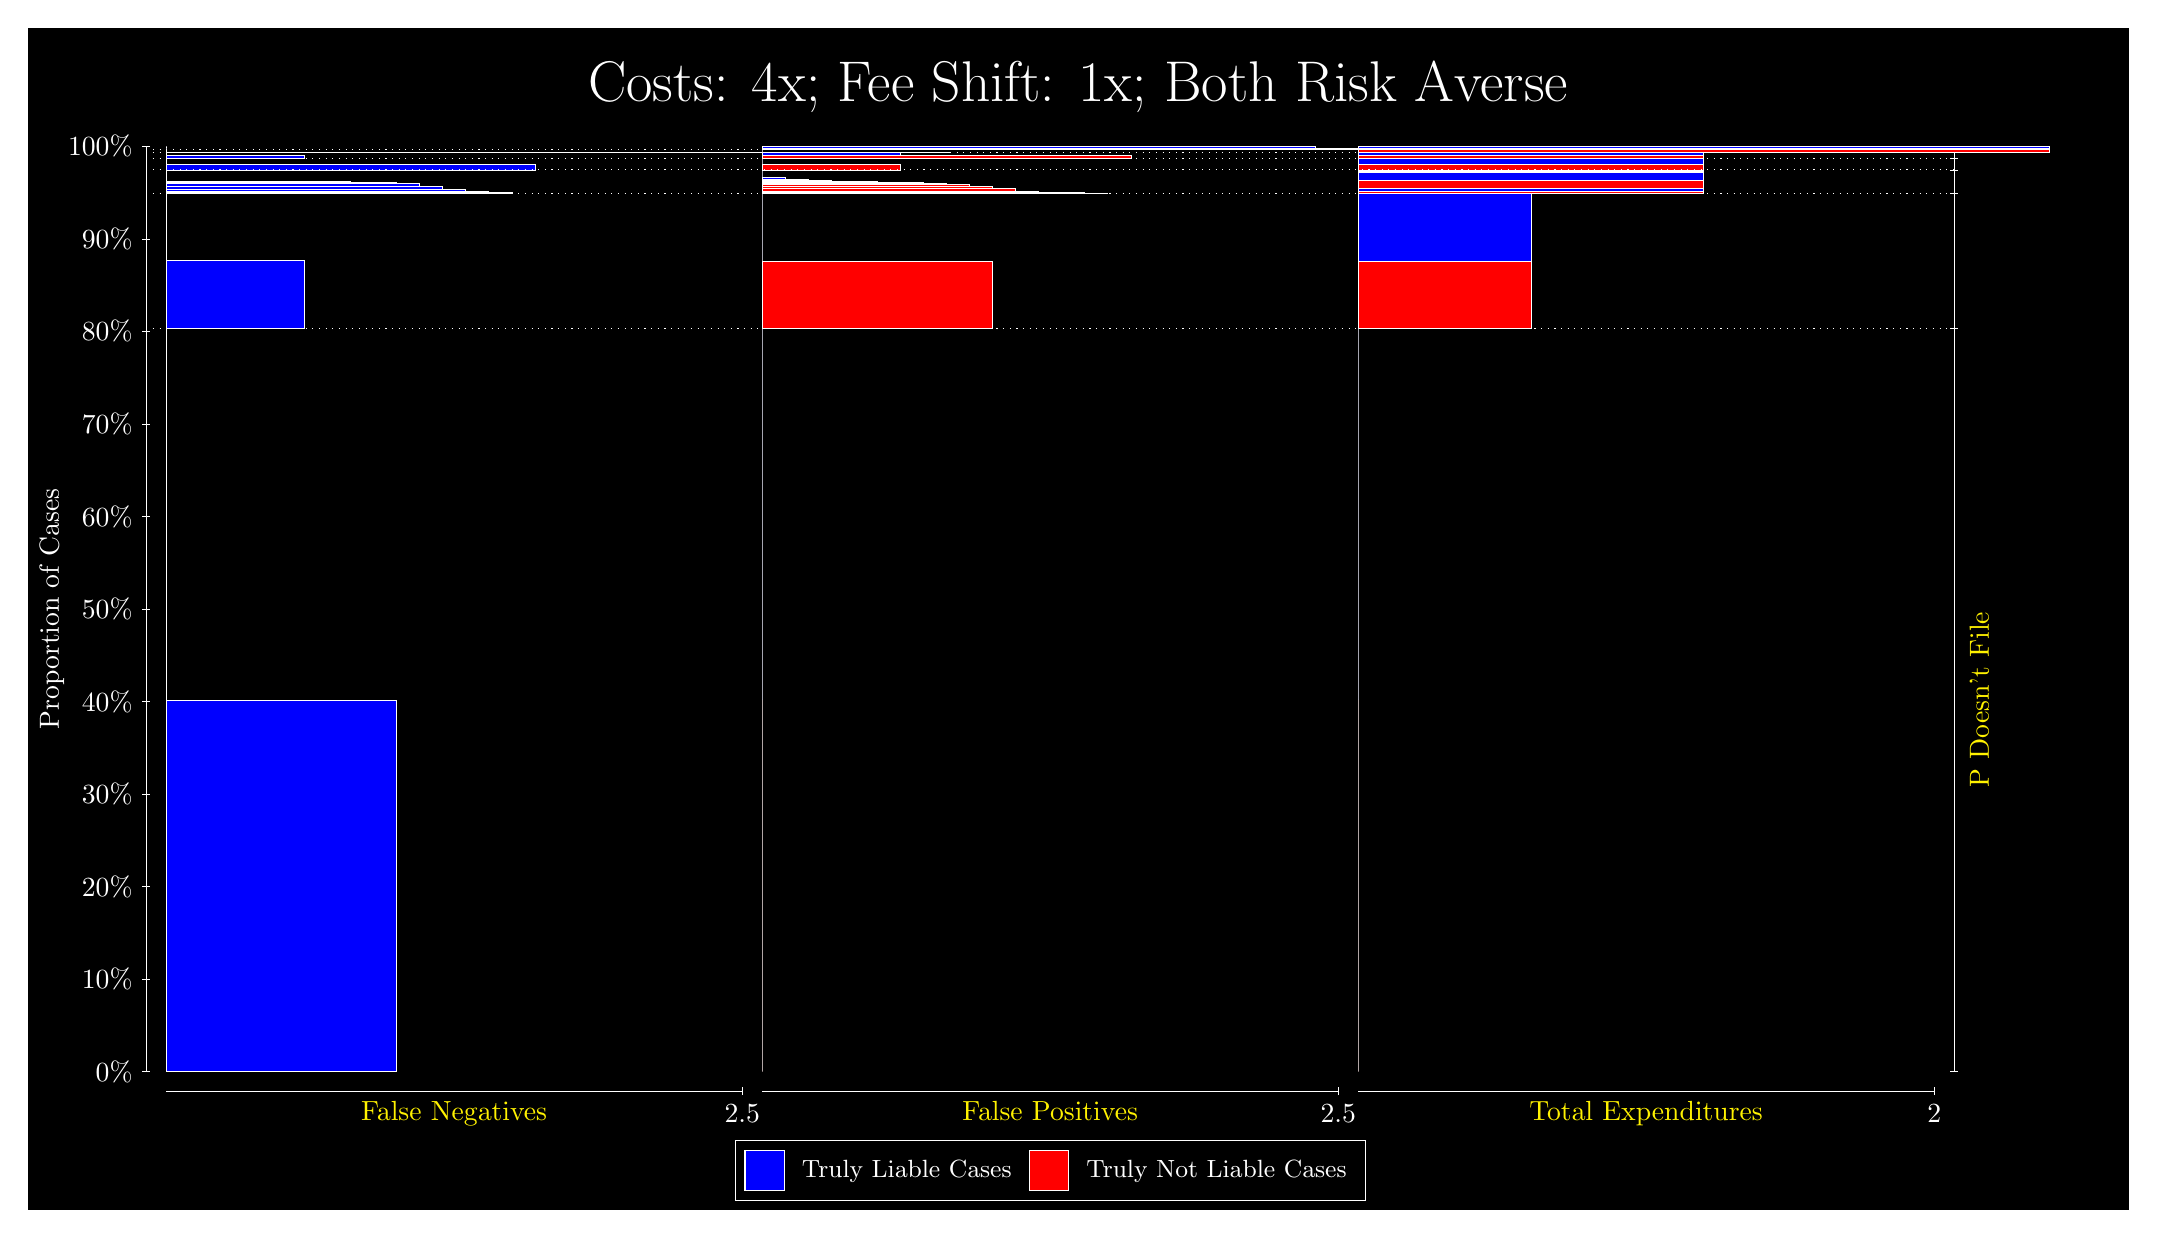
\begin{tikzpicture}
\draw[fill=black] (0,0) rectangle (26.667,15);
\draw[text=white] (0,13.5) rectangle (26.667,15) node[midway] {\huge Costs: 4x; Fee Shift: 1x; Both Risk Averse};
\draw[white, very thin] (1.5,1.75) -- (1.5,13.5);
\node[rotate=90, text=white, anchor=center] at (0.3, 7.625) {Proportion of Cases};
\draw[white, very thin] (1.45,1.75) -- (1.55,1.75);
\node[text=white, anchor=east] at (1.45, 1.75) {0\%};
\draw[white, very thin] (1.45,2.925) -- (1.55,2.925);
\node[text=white, anchor=east] at (1.45, 2.925) {10\%};
\draw[white, very thin] (1.45,4.1) -- (1.55,4.1);
\node[text=white, anchor=east] at (1.45, 4.1) {20\%};
\draw[white, very thin] (1.45,5.275) -- (1.55,5.275);
\node[text=white, anchor=east] at (1.45, 5.275) {30\%};
\draw[white, very thin] (1.45,6.45) -- (1.55,6.45);
\node[text=white, anchor=east] at (1.45, 6.45) {40\%};
\draw[white, very thin] (1.45,7.625) -- (1.55,7.625);
\node[text=white, anchor=east] at (1.45, 7.625) {50\%};
\draw[white, very thin] (1.45,8.8) -- (1.55,8.8);
\node[text=white, anchor=east] at (1.45, 8.8) {60\%};
\draw[white, very thin] (1.45,9.975) -- (1.55,9.975);
\node[text=white, anchor=east] at (1.45, 9.975) {70\%};
\draw[white, very thin] (1.45,11.15) -- (1.55,11.15);
\node[text=white, anchor=east] at (1.45, 11.15) {80\%};
\draw[white, very thin] (1.45,12.325) -- (1.55,12.325);
\node[text=white, anchor=east] at (1.45, 12.325) {90\%};
\draw[white, very thin] (1.45,13.5) -- (1.55,13.5);
\node[text=white, anchor=east] at (1.45, 13.5) {100\%};

\draw[white, very thin] (24.457,1.75) -- (24.457,13.5);
\draw[white, very thin] (24.407,1.75) -- (24.507,1.75);
\node[anchor=west] at (24.407, 1.75) {};
\draw[white, very thin] (24.407,11.191) -- (24.507,11.191);
\node[anchor=west] at (24.407, 11.191) {};
\draw[white, very thin] (24.407,12.903) -- (24.507,12.903);
\node[anchor=west] at (24.407, 12.903) {};
\draw[white, very thin] (24.407,13.201) -- (24.507,13.201);
\node[anchor=west] at (24.407, 13.201) {};
\draw[white, very thin] (24.407,13.343) -- (24.507,13.343);
\node[anchor=west] at (24.407, 13.343) {};
\draw[white, very thin] (24.407,13.421) -- (24.507,13.421);
\node[anchor=west] at (24.407, 13.421) {};
\draw[white, very thin] (24.407,13.465) -- (24.507,13.465);
\node[anchor=west] at (24.407, 13.465) {};
\draw[white, very thin] (24.407,13.5) -- (24.507,13.5);
\node[anchor=west] at (24.407, 13.5) {};

\draw[white, very thin, fill=blue] (1.75,1.75) rectangle (4.6775,6.4706);
\draw[white, very thin, fill=red] (1.75,6.4706) rectangle (1.75,11.191);
\draw[white, very thin, fill=blue] (1.75,11.191) rectangle (3.5065,12.052);
\draw[white, very thin, fill=red] (1.75,12.052) rectangle (1.75,12.903);
\draw[white, very thin, fill=blue] (1.75,12.903) rectangle (6.1413,12.917);
\draw[white, very thin, fill=blue] (1.75,12.917) rectangle (5.8486,12.925);
\draw[white, very thin, fill=blue] (1.75,12.925) rectangle (5.5558,12.958);
\draw[white, very thin, fill=blue] (1.75,12.958) rectangle (5.2631,12.993);
\draw[white, very thin, fill=blue] (1.75,12.993) rectangle (4.9703,13.027);
\draw[white, very thin, fill=blue] (1.75,13.027) rectangle (4.6775,13.038);
\draw[white, very thin, fill=blue] (1.75,13.038) rectangle (4.3848,13.047);
\draw[white, very thin, fill=blue] (1.75,13.047) rectangle (4.092,13.051);
\draw[white, very thin, fill=blue] (1.75,13.051) rectangle (3.7993,13.055);
\draw[white, very thin, fill=red] (1.75,13.055) rectangle (1.75,13.201);
\draw[white, very thin, fill=blue] (1.75,13.201) rectangle (6.4341,13.266);
\draw[white, very thin, fill=red] (1.75,13.266) rectangle (1.75,13.343);
\draw[white, very thin, fill=blue] (1.75,13.343) rectangle (3.5065,13.384);
\draw[white, very thin, fill=red] (1.75,13.384) rectangle (1.75,13.421);
\draw[white, very thin, fill=blue] (1.75,13.421) rectangle (11.704,13.428);
\draw[white, very thin, fill=red] (1.75,13.428) rectangle (1.75,13.465);
\draw[white, very thin, fill=red] (1.75,13.465) rectangle (1.75,13.472);
\draw[white, very thin, fill=blue] (1.75,13.472) rectangle (1.75,13.5);
\draw[white, very thin, fill=red] (9.3189,1.75) rectangle (9.3189,6.4707);
\draw[white, very thin, fill=blue] (9.3189,6.4707) rectangle (9.3189,11.191);
\draw[white, very thin, fill=red] (9.3189,11.191) rectangle (12.246,12.042);
\draw[white, very thin, fill=blue] (9.3189,12.042) rectangle (9.3189,12.903);
\draw[white, very thin, fill=red] (9.3189,12.903) rectangle (13.71,12.907);
\draw[white, very thin, fill=red] (9.3189,12.907) rectangle (13.417,12.911);
\draw[white, very thin, fill=red] (9.3189,12.911) rectangle (13.125,12.919);
\draw[white, very thin, fill=red] (9.3189,12.919) rectangle (12.832,12.93);
\draw[white, very thin, fill=red] (9.3189,12.93) rectangle (12.539,12.963);
\draw[white, very thin, fill=red] (9.3189,12.963) rectangle (12.246,12.994);
\draw[white, very thin, fill=red] (9.3189,12.994) rectangle (11.954,13.023);
\draw[white, very thin, fill=red] (9.3189,13.023) rectangle (11.661,13.03);
\draw[white, very thin, fill=red] (9.3189,13.03) rectangle (11.368,13.049);
\draw[white, very thin, fill=blue] (9.3189,13.049) rectangle (10.783,13.053);
\draw[white, very thin, fill=blue] (9.3189,13.053) rectangle (10.49,13.057);
\draw[white, very thin, fill=blue] (9.3189,13.057) rectangle (10.197,13.066);
\draw[white, very thin, fill=blue] (9.3189,13.066) rectangle (9.9044,13.077);
\draw[white, very thin, fill=blue] (9.3189,13.077) rectangle (9.6116,13.111);
\draw[white, very thin, fill=blue] (9.3189,13.111) rectangle (9.3189,13.201);
\draw[white, very thin, fill=red] (9.3189,13.201) rectangle (11.075,13.278);
\draw[white, very thin, fill=blue] (9.3189,13.278) rectangle (9.3189,13.343);
\draw[white, very thin, fill=red] (9.3189,13.343) rectangle (14.003,13.38);
\draw[white, very thin, fill=blue] (9.3189,13.38) rectangle (11.075,13.421);
\draw[white, very thin, fill=red] (9.3189,13.421) rectangle (9.3189,13.457);
\draw[white, very thin, fill=blue] (9.3189,13.457) rectangle (9.3189,13.465);
\draw[white, very thin, fill=red] (9.3189,13.465) rectangle (19.273,13.472);
\draw[white, very thin, fill=blue] (9.3189,13.472) rectangle (16.345,13.5);
\draw[white, very thin, fill=red] (16.888,1.75) rectangle (16.888,6.4707);
\draw[white, very thin, fill=blue] (16.888,6.4707) rectangle (16.888,11.191);
\draw[white, very thin, fill=red] (16.888,11.191) rectangle (19.083,12.042);
\draw[white, very thin, fill=blue] (16.888,12.042) rectangle (19.083,12.903);
\draw[white, very thin, fill=red] (16.888,12.903) rectangle (21.279,12.935);
\draw[white, very thin, fill=blue] (16.888,12.935) rectangle (21.279,12.969);
\draw[white, very thin, fill=red] (16.888,12.969) rectangle (21.279,13.071);
\draw[white, very thin, fill=blue] (16.888,13.071) rectangle (21.279,13.176);
\draw[white, very thin, fill=red] (16.888,13.176) rectangle (21.279,13.189);
\draw[white, very thin, fill=blue] (16.888,13.189) rectangle (21.279,13.201);
\draw[white, very thin, fill=red] (16.888,13.201) rectangle (21.279,13.278);
\draw[white, very thin, fill=blue] (16.888,13.278) rectangle (21.279,13.343);
\draw[white, very thin, fill=red] (16.888,13.343) rectangle (21.279,13.38);
\draw[white, very thin, fill=blue] (16.888,13.38) rectangle (21.279,13.421);
\draw[white, very thin, fill=red] (16.888,13.421) rectangle (25.67,13.457);
\draw[white, very thin, fill=blue] (16.888,13.457) rectangle (25.67,13.465);
\draw[white, very thin, fill=red] (16.888,13.465) rectangle (25.67,13.472);
\draw[white, very thin, fill=blue] (16.888,13.472) rectangle (25.67,13.5);
\draw[white, dotted] (1.5,11.191) -- (24.457,11.191);
\draw[white, dotted] (1.5,12.903) -- (24.457,12.903);
\draw[white, dotted] (1.5,13.201) -- (24.457,13.201);
\draw[white, dotted] (1.5,13.343) -- (24.457,13.343);
\draw[white, dotted] (1.5,13.421) -- (24.457,13.421);
\draw[white, dotted] (1.5,13.465) -- (24.457,13.465);
\draw[white, very thin] (1.75,1.5) -- (9.0689,1.5);
\node[text=yellow, anchor=north] at (5.4094, 1.5) {False Negatives};
\draw[white, very thin] (9.0689,1.45) -- (9.0689,1.55);
\node[text=white, anchor=north] at (9.0689, 1.45) {2.5};

\draw[white, very thin] (9.3189,1.5) -- (16.638,1.5);
\node[text=yellow, anchor=north] at (12.978, 1.5) {False Positives};
\draw[white, very thin] (16.638,1.45) -- (16.638,1.55);
\node[text=white, anchor=north] at (16.638, 1.45) {2.5};

\draw[white, very thin] (16.888,1.5) -- (24.207,1.5);
\node[text=yellow, anchor=north] at (20.547, 1.5) {Total Expenditures};
\draw[white, very thin] (24.207,1.45) -- (24.207,1.55);
\node[text=white, anchor=north] at (24.207, 1.45) {2};

\node[text=yellow, centered, rotate=90] at (24.777, 6.4706) {P Doesn't File};







\draw (12.978300999999998,1.5) node[draw=none] (baseCoordinate) {};
\begin{scope}[align=center]
        \matrix[scale=0.5, draw=white, below=0.5cm of baseCoordinate, nodes={draw}, column sep=0.1cm]{
            \node[rectangle, draw, minimum width=0.5cm, minimum height=0.5cm, fill=blue] {}; &
            \node[draw=none, font=\small, text=white] (B) {Truly Liable Cases}; &
            \node[rectangle, draw, minimum width=0.5cm, minimum height=0.5cm, fill=red] {}; &
            \node[draw=none, font=\small, text=white] (B) {Truly Not Liable Cases}; \\
            };
\end{scope}

\end{tikzpicture}
\end{document}